\section{Dynamic Scalable State Machine Replication}

In this section, we introduce Dynamic SSMR, discuss performance optimizations, and argue about D-SSMR's correctness.

\subsection{General idea}
\label{sec:generalidea}

S-SMR divides the state variables $v$ into $P$ partitions $p_1, ..., p_P$, where for each $p_i$, $p_i \subseteq V$, and each variable $v$ in $V$ has to be assigned to at least one partition and define $part(v)$ as the partitions that hold $v$. Each partition $p_i$ is replicated by servers in group $s_i$. For brevity, the server $s$ belongs to $p_i$ with the meaning that $s \in S_i$, and say that client $c$ multicasts command $C$ to partition $P_i$ means that $c$ multicasts $C$ to group $S_i$.

To execute command $C$, the client multicasts $C$ to all partitions that hold a variable read or updated by $C$.
Consequently, the client must be able to determine the partitions accessed by $C$, denoted by $part(C)$. If the client cannot accurately estimate which partitions are accessed by $C$, it must determine a superset of these partitions, in the worst case assuming all partitions.
In order for clients to provide a close approximation to the command's actually accessed partitions, there is an oracle that tells the client which partitions should receive each command.

Dynamic SSMR improves on SSMR implementation by adding a central Oracle which has the information of all state variables $V$, as well as provides a mechanism of controlling the access to those variable that ensure linearizability. 

We distinguish between three operation types: $read(v)$, an operation that reads the value of a state variable, $v$, $create(v, P)$, an operation that create a state variable at a specific partition P, and $move(v, p_n)$, an operation that move $v$ to partition $p_n$,

Consider the execution depicted in Figure~\ref{fig:read}~(a), where state variables $x$ is created on partition $p_1$ in the middle of the execution of SSMR. Command $C_1(x)$ and $C_3(x)$ reads the value of $x$, $C_2(x,p1)$ create $x$ on partition $p_1$. Client a first multicasts query to the $Oracle$ for location of $x$, which is not available at that time, hence $Oracle$ return empty result, which tell client a to end the execution. Client b then wants to create variable $x$ on $p_1$, before sending actual creating command, client b also multicasts query to $Oracle$ to get the involved partition (eg., $p_1$), then multicasts $C_2(x,p1)$ to both $Oracle$ and $p_1$. Oracle will update information of $x$, and $p_1$ will execute create $x$ command. From then, for every read command to $x$ (eg., $C_3(x)$), $Oracle$ could answer with partition $p_1$ which is the one holds $x$.

\begin{figure*}
\begin{minipage}[b]{1.0\linewidth} % A minipage that covers the whole width of the page
\centering
      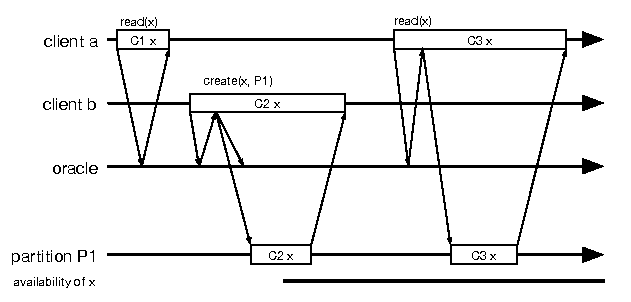
\includegraphics[width=0.6\linewidth]{figures/read_common}
\end{minipage}
\caption{Execution flow of D-SSMR with $create$ command}
\label{fig:read}
\end{figure*}

In the following figures~(\ref{fig:readoverlap}b, \ref{fig:readoverlap}c), where read command $C_1(x)$ comes in the middle of the execution of create command $C_2(x,p1)$, while the query of $C_1(x)$ comes after multicasts command of $C_2(x,p1)$. With the knowledge of $x$, Oracle response to the query with a positive answer, therefore there are possibilities that the read command either comes during (eg., fig.~\ref{fig:readoverlap}b) or before (eg., fig.~\ref{fig:readoverlap}c) the execution of actual write command. The SSMR model avoid the problem described in figure~\ref{fig:readoverlap}~(b) by ensuring that the execution of every command is atomic (eg., for every server $s$ in partition $P$ that executes $C$, there is a server $r$ in every $P' \in part(C)$ such that $delivery(C,r) < end(C,s)$. Intuitively, this condition guarantees that the execution of $C$ at $P$ and $P'$ overlap in time.) With the problem figure~\ref{fig:readoverlap}~(c) TODO: explain

\begin{figure*}
\begin{minipage}[b]{1.0\linewidth} % A minipage that covers the whole width of the page
\centering
      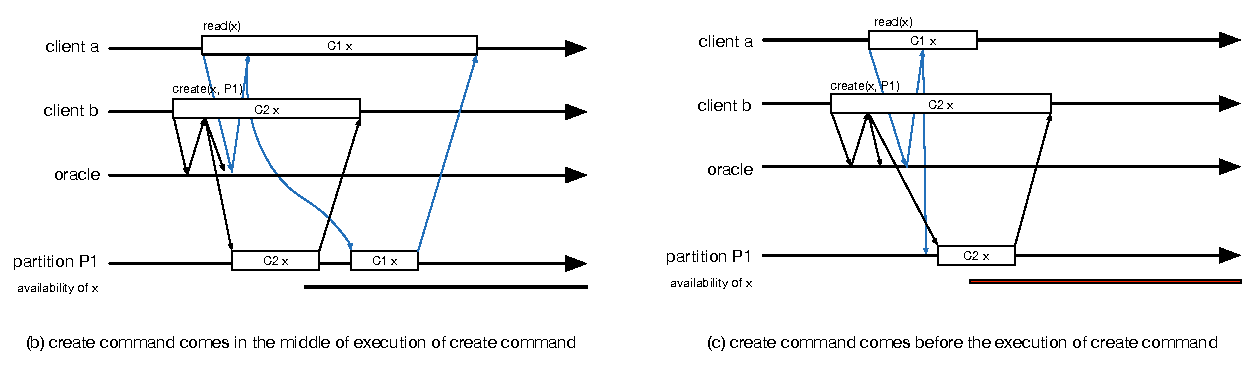
\includegraphics[width=1\linewidth]{figures/read_overlap}
\end{minipage}
\caption{Execution flow of D-SSMR with overlapping commands}
\label{fig:readoverlap}
\end{figure*}